\begin{dang}{Khảo sát và vẽ đồ thị hàm số phân thức hữu tỉ bậc II/I}
	\begin{itemize}
		\item[\iconCH] \indamm{Bước 1.} Tập xác định $D=\mathbb{R}\backslash \left\{-\dfrac{n}{m}\right\}$.
		\item [\iconCH] \indamm{Bước 2.} Khảo sát sự biến thiên của hàm số
		\begin{itemize}
			\item Tính đạo hàm $y'=\dfrac{am\cdot x^2+2an\cdot x + b.n - m.c}{(mx+n)^2}$. Giải $y'=0 \Leftrightarrow am\cdot x^2+2an\cdot x + b.n - m.c=0$, tìm nghiệm.
			\item Tìm các giới hạn tại vô cực, giới hạn vô cực và tìm tiệm cận của đồ thị hàm số.
			\item Lập bảng biến thiên; xác định chiều biến thiên và cực trị của hàm số.
		\end{itemize}
		\item [\iconCH] \indamm{Bước 3.} Cho thêm điểm và vẽ đồ thị của hàm số dựa vào bảng biến thiên.
	\end{itemize}
\end{dang}
\boxmini{BÀI TẬP TỰ LUẬN}
\begin{vd}
	Khảo sát sự biến thiên và vẽ đồ thị các hàm số sau:
	\begin{tasks}(3)
		\task $ y = \dfrac{x^2+ 2x - 2}{x - 1}$;
		\task $y=-x+2-\dfrac{1}{x+1}$;
		\task $y=\dfrac{-x^2-3x+4}{x+2}$.
	\end{tasks}
\loigiai{
\begin{enumerate}[a)]
	\item Ta viết lại hàm số $ y = \dfrac{x^2+ 2x - 2}{x - 1}=x+3+\dfrac{1}{x-1}$.\\
	Tập xác định: $D = \mathbb{R} \setminus \left\{ 1 \right\}$.\\
	Sự biến thiên:
	\begin{itemize}
		\item [$\bullet$] Đạo hàm $y'= \dfrac{x^2 - 2x}{(x - 1)^2}$; $y' = 0 \Leftrightarrow x = 0$  hoặc $x = 2$.
		\item [$\bullet$] Giới hạn và tiệm cận:\\
		$\displaystyle\lim \limits{n \to +\infty}_{x \rightarrow-\infty} y=-\infty,\, \displaystyle\lim \limits{n \to +\infty}_{x \rightarrow +\infty} y=+\infty$.\\
		$\displaystyle\lim \limits{n \to +\infty}_{x \rightarrow 1^{-}} y= -\infty,\, \displaystyle\lim \limits{n \to +\infty}_{x \rightarrow 1^{+}} y=+\infty$. Suy ra $x=1$ là tiệm cận đứng.\\
		$\displaystyle\lim \limits{n \to +\infty}_{x \rightarrow -\infty} \left(y-(x+3) \right) = 0,\, \displaystyle\lim \limits{n \to +\infty}_{x \rightarrow +\infty} \left(y-(x+3) \right) = 0$. Suy ra $y=x+3$ là tiệm cận xiên.
		\item [$\bullet$] Bảng biến thiên:
		\begin{center}
			
\begin{tikzpicture}[scale=1, font=\footnotesize, line join=round, line cap=round, >=stealth]
				\tikzset{double style/.append style = {draw=\tkzTabDefaultWritingColor,double=\tkzTabDefaultBackgroundColor,double distance=2pt}}
				\tkzTabInit[nocadre=false,lgt=1.2,espcl=2.2,deltacl=0.6]
				{$x$ /0.6,$y'$ /0.6,$y$ /1.6}
				{$-\infty$,$0$,$1$,$2$,$+\infty$}
				\tkzTabLine{,+,0,-,d,-,0,+,}
				\tkzTabVar{-/$-\infty$,+/$2$,-D+/$-\infty$/$+\infty$,-/$6$,+/$+\infty$}
			\end{tikzpicture}
		\end{center}
	Hàm số đồng biến trên khoảng $(-\infty;0)$ và $(2;+\infty)$; nghịch biến trên khoảng $(0;1)$ và $(1;2)$.\\
	Hàm số đạt cực tiểu tại $x = 2$  và ${y_{CT}} = 6$ .\\
	Hàm số đạt cực đại tại $x = 0$ và ${y_{CĐ}} = 2$ .\\
	\end{itemize}
	Đồ thị:\\
	\immini{
		\begin{itemize}
			\item [$\bullet$] Đồ thị hàm số giao với trục $Ox$ tại điểm $(-1+\sqrt{3}; 0)$ và điểm $(-1-\sqrt{3}; 0)$.
			\item [$\bullet$] Đồ thị nhận $I(1;4)$ làm tâm đối xứng.
		\end{itemize}
	}{
	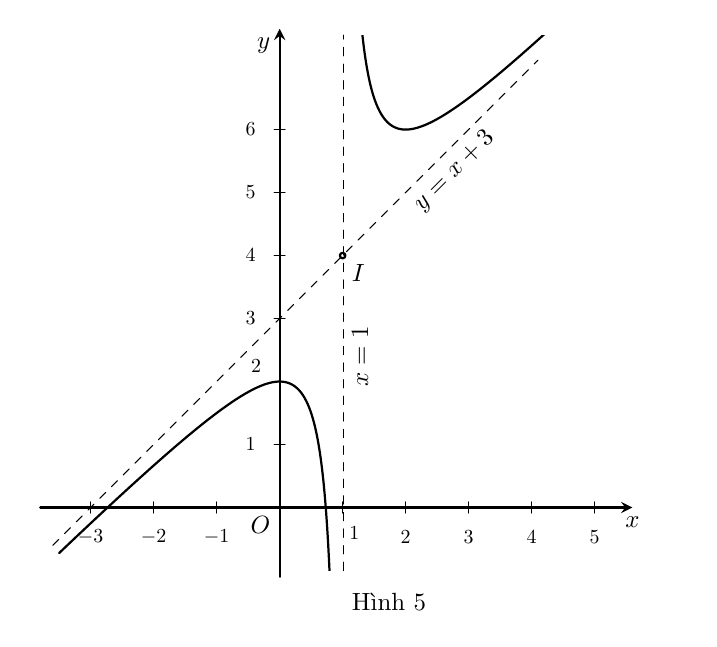
\begin{tikzpicture}[line join=round, line cap=round,>=stealth,thick,x=0.8cm,y=0.8cm]
		\tikzset{every node/.style={scale=0.9}}
		\draw[->] (-3.8,0)--(5.6,0) node[below] {$x$};
		\draw[->] (0,-1.1)--(0,7.6) node[below left] {$y$};
		\draw (0,0) node [below left] {$O$};
		\draw (1,4) circle (1pt) node [below right] {$I$};
		\draw (1,-1.5) node [right] {Hình 5};
		\draw[dashed,thin] (1.01,-1)--(1.01,7.5) node [pos=0.4,sloped,black,below] {$x=1$} ;
		\begin{scope}
			\clip (-4,-1) rectangle (6.5,7.5);
			\draw[samples=200,domain=-3.5:0.99,smooth,variable=\x] plot (\x,{(1*((\x)^2)+2*(\x)+-2)/(1*(\x)+-1)});
			\draw[samples=200,domain=1.01:6,smooth,variable=\x] plot (\x,{(1*((\x)^2)+2*(\x)+-2)/(1*(\x)+-1)});
			\draw[dashed,thin] (-3.6,-0.6)--(4.1,7.1) node [pos=0.8,sloped,black,below] {$y=x+3$};
		\end{scope}
		\foreach \x/\g in {-3/-90,-2/-90,-1/-90,1/-60,2/-90,3/-90,4/-90,5/-90}
		\draw[thin] (\x,2pt)--(\x,-2pt) + (\g:3mm) node [scale=0.8] {$\x$};
		%Vẽ các điểm trên trục Oy
		\foreach \y/\g in {1/180,2/140,3/180,6/180,4/180,5/180}
		\draw[thin] (2pt,\y)--(-2pt,\y) + (\g:3mm) node [scale=0.8] {$\y$};
\end{tikzpicture}}

	\item Tập xác định: $\mathscr{D}=\mathbb{R} \backslash\{-1\}$.\\
	Sự biến thiên:
	\begin{itemize}
		\item [$\bullet$] Đạo hàm $y'=-1+\dfrac{1}{(x+1)^2}$, $y'=0\Leftrightarrow x=-2$ hoặc $x=0$.
		\item [$\bullet$] Giới hạn và tiệm cận:\\
		\begin{itemize}
			\item $\lim\limits_{x \rightarrow +\infty} y= -\infty, \lim\limits_{x \rightarrow -\infty} y= +\infty$.
			\item $\lim\limits_{x \rightarrow (-1)^{-}} y= +\infty, \lim\limits_{x \rightarrow (-1)^{+}} y= -\infty$.
		\end{itemize}
		Do đó, đường thẳng $x=-1$ là tiệm cận đứng của đồ thị hàm số.
		\begin{itemize}
			\item $\lim\limits_{x \rightarrow+\infty}[y - (-x+2)]=\lim\limits_{x \rightarrow +\infty} \dfrac{-1}{x+1}=0$,
			\item $ \lim\limits_{x \rightarrow-\infty}[y - (-x+2)]=\lim\limits_{x \rightarrow +\infty} \dfrac{-1}{x+1}=0$.
		\end{itemize}
		Do đó, đường thẳng $y= -x+2 $ là tiệm cận xiên của đồ thị hàm số.
		\item [$\bullet$] Bảng biến thiên:
		\begin{center}
			
\begin{tikzpicture}
				\tikzset{double style/.append style = {draw=\tkzTabDefaultWritingColor,double=\tkzTabDefaultBackgroundColor,double distance=2pt}}
				\tkzTabInit[lgt=1.2, espcl=2.5, deltacl=0.6]
				{$x$/0.6, $y'$/0.6, $y$/2}
				{$-\infty$, $-2$, $-1$, $0$, $+\infty$}
				\tkzTabLine{, -, 0, +, d, +, 0, -, }
				\tkzTabVar{+/$+\infty$, -/$5$, +D-/$+\infty$/$-\infty$, +/$1$, -/$-\infty$}
			\end{tikzpicture}
		\end{center}
		Hàm số đồng biến trên các khoảng $(-2;-1)$, $(-1;0)$ và nghịch biến trên các khoảng $(-\infty;-2)$, $(0;+\infty)$.\\
		Hàm số đạt cực tiểu tại $x=-2$, $y_{_\text{CT}}=5$; đạt cực đại tại $x=0$, $y_{_\text{CĐ}}=1$.\\
	\end{itemize}
	Đồ thị:\\
	\immini{
		\begin{itemize}
			\item [$\bullet$] Đồ thị hàm số qua các điểm $\left(-3;-\dfrac{11}{2} \right)$, $\left(3;-\dfrac{5}{4} \right)$.
			\item [$\bullet$] Đồ thị nhận $I(-1;3)$ làm tâm đối xứng.
		\end{itemize}
	}{
		\begin{tikzpicture}[>=stealth, scale=0.6, font=\footnotesize,x=1cm,y=1cm]
			\draw[->] (-5,0)--(5,0) node[below] {$x$};
			\draw[->] (0,-4)--(0,8.5) node[left] {$y$};
			\draw[domain=-0.85:3.8, smooth] plot (\x, {-(\x)^2+(\x)+1)/(\x+1)});
			\draw[domain=-4:-1.2, smooth] plot (\x, {-(\x)^2+(\x)+1)/(\x+1)});
			\draw[domain=-4.5:4, smooth] plot (\x, {-\x+2});
			\draw (-1,-4)--(-1,8.2);
			\draw[fill=black] (0,0) node[below left=-0.1] {$O$} circle (1.2pt);
			\draw[fill=black] (1,0) node[below] {$1$} circle (1.2pt);
			\draw[fill=black] (2,0) node[above] {$2$} circle (1.2pt);
			\draw[fill=black] (-1,0) node[above] {$-1$} circle (1.2pt);
			\draw[fill=black] (-2,0) node[below ] {$-2$} circle (1.2pt);
			\draw[fill=black] (3,0) node[above ] {$3$} circle (1.2pt);
			%	\draw[fill=black] (-4,0) node[below] {$-4$} circle (1.2pt);
			\draw[fill=black] (0,5) node[right] {$5$} circle (1.2pt);
			%		\draw[fill=black] (0,17) node[right] {$17$} circle (1.2pt);
			\draw[fill=black] (0,-1.25) node[ left] {$-\dfrac{5}{4}$} circle (1.2pt);
			\draw[fill=black] (0,1) node[above right] {$1$} circle (1.2pt);
			\draw[dashed] (-2,0)--(-2,5)--(0,5) (3,0)--(3,-1.25)--(0,-1.25) (1,0)--(1,0.5)--(0,0.5) ;
	\end{tikzpicture}}
	
	\item Ta viết lại hàm số $ y = \dfrac{x^2+ 2x - 2}{x - 1}=x+3+\dfrac{1}{x-1}$.\\
	Tập xác định: $D=\mathbb{R} \setminus\{-2\}$.\\
	Sự biến thiên:
	\begin{itemize}
		\item [$\bullet$] Đạo hàm Đạo hàm $y'=\dfrac{-x^2-4x-10}{(x+2)^2}<0$, với mọi $x \ne -2$.
		\item [$\bullet$] Giới hạn và tiệm cận:\\
		$$
		\lim\limits_{x \to-\infty} y=\lim\limits_{x \to-\infty} \dfrac{-x^2-3 x+4}{x+2}=+\infty; \lim\limits_{x \to+\infty} y=\lim\limits_{x \to+\infty} \dfrac{-x^2-3 x+4}{x+2}=-\infty.
		$$		
		Ta có 
		\begin{itemize}
			\item $a=\lim\limits_{x \to+\infty} \dfrac{-x^2-3x+4}{x^2+2x}=-1$.
			\item $b=\lim\limits_{x \to+\infty}\left[\dfrac{-x^2-3x+4}{x+2}-(-1) x\right]=\lim\limits_{x \to+\infty}\left(\dfrac{-x+4}{x+2}\right)=-1$.
		\end{itemize}	
		Suy ra đường thẳng $y=-x-1$ là tiệm cận xiên của đồ thị hàm số.\\		
		Ta có $\lim\limits_{x \to-2^{-}} y=\lim\limits_{x \to-2^{-}} \dfrac{-x^2-3x+4}{x+2}=-\infty; \lim\limits_{x \to-2^{+}} y=\lim\limits_{x \to-2^{+}} \dfrac{-x^2-3x+4}{x+2}=+\infty$. Suy ra đường thẳng $x=-2$ là tiệm cận đứng của đồ thị hàm số.
		\item [$\bullet$] Bảng biến thiên:
		\begin{center}
			
\begin{tikzpicture}
				\tikzset{double style/.append style = {draw=\tkzTabDefaultWritingColor,double=\tkzTabDefaultBackgroundColor,double distance=2pt}}
				\tkzTabInit[nocadre=false,espcl=3,lgt=1.5]
				{$x$/0.7,$y'$/0.7,$y$/2.1}
				{$-\infty$,$-2$,$+\infty$}
				\tkzTabLine{,-,d,-,}
				\tkzTabVar{+/$+\infty$,-D+/$-\infty$/$+\infty$,-/$-\infty$}
			\end{tikzpicture}
		\end{center}
		Hàm số nghịch biến trên khoảng $(-\infty;-2)$ và $(-2;+\infty)$.\\
		Hàm số không có cực trị.
	\end{itemize}
	Đồ thị:\\
	\immini{
		\begin{itemize}
			\item [$\bullet$] Đồ thị hàm số giao với trục $Ox$ tại điểm $(-4; 0)$ và điểm $(1; 0)$.
			\item [$\bullet$] Đồ thị nhận $I(-2;1)$ làm tâm đối xứng.
		\end{itemize}
	}{
		\begin{tikzpicture}[>=stealth, scale=0.6, font=\footnotesize]
			\draw[->] (-7,0)--(5.5,0) node[below] {$x$};
			\draw[->] (0,-7)--(0,7) node[left] {$y$};
			\draw[domain=-1.1:5, smooth] plot (\x, {-(\x)^2-3*(\x)+4)/(\x+2)});
			\draw[domain=-6.4:-2.7, smooth] plot (\x, {-(\x)^2-3*(\x)+4)/(\x+2)});
			\draw[domain=-6:5, smooth] plot (\x, {-\x-1});
			\draw (-2,-7)--(-2,7);
			\draw[fill=black] (0,0) node[below left=-0.1] {$O$} circle (1.2pt);
			\draw[fill=black] (1,0) node[below] {$1$} circle (1.2pt);
			\draw[fill=black] (-1,0) node[below left] {$-1$} circle (1.2pt);
			\draw[fill=black] (2,0) node[below right=0 and -0.1] {$2$} circle (1.2pt);
			\draw[fill=black] (4,0) node[above] {$4$} circle (1.2pt);
			\draw[fill=black] (0,6) node[right] {$6$} circle (1.2pt);
			\draw[fill=black] (0,2) node[below left] {$2$} circle (1.2pt);
			\draw[fill=black] (0,-2.8) node[left] {$-\dfrac{14}{5}$} circle (1.2pt);
			\draw[fill=black] (0,-4) node[left] {$-4$} circle (1.2pt);
			\draw[dashed] (3,0)--(3,-2.8)--(0,-2.8) (4,0)--(4,-4)--(0,-4) (-1,0)--(-1,6)--(0,6);
			\node [above=-1mm, fill=white,font=\footnotesize] at (1.5,-7) {\it Hình $6$};
	\end{tikzpicture}}

\end{enumerate}}
\end{vd}

\boxmini{BÀI TẬP TRẮC NGHIỆM}
\ind{PHẦN I.} \inden{Câu trắc nghiệm nhiều phương án lựa chọn. Mỗi câu hỏi học sinh chỉ chọn một phương án.}\\
\setcounter{ex}{0}
\Opensolutionfile{ans}[ans/2D1-B4-d3-1]
\begin{ex}
	\immini{Bảng biến thiên sau là của một trong bốn hàm số sau. Hỏi đó là hàm số nào?
	\choice
	{$y=\dfrac{x^2-3x+4}{-x-4}$}
	{\True $y=\dfrac{x^2-4x+4}{-x-4}$}
	{$y=\dfrac{x^2-5x+4}{x+4}$}
	{$y=\dfrac{x^2-4x+4}{x+4}$}}{
	
\begin{tikzpicture}
		\tikzset{double style/.append style = {draw=\tkzTabDefaultWritingColor,double=\tkzTabDefaultBackgroundColor,double distance=2pt}}
		\tkzTabInit[nocadre=false,lgt=1,espcl=1.6]
		{$x$ /0.6,$y'$ /0.6,$y$ /1.5}
		{$-\infty$,$-10$,$-4$,$2$,$+\infty$}
		\tkzTabLine{,-,$0$,+,d,+,$0$,-,}
		\tkzTabVar{+/$+\infty$,-/$24$,+D-/$+\infty$/$-\infty$,+/$0$,-/$-\infty$}
	\end{tikzpicture}
}
\loigiai{
}
\end{ex}

\begin{ex}
	\immini{Bảng biến thiên sau là của một trong bốn hàm số sau. Hỏi đó là hàm số nào?
		\choice
		{$y=\dfrac{x^2-4x+3}{x-3}$}
		{$y=\dfrac{-x^2-x+2}{x-3}$}
		{\True $y=\dfrac{-x^2+x+2}{x-3}$}
		{$y=\dfrac{x^2-4x+4}{-x+3}$}}{
		
\begin{tikzpicture}
			\tikzset{double style/.append style = {draw=\tkzTabDefaultWritingColor,double=\tkzTabDefaultBackgroundColor,double distance=2pt}}
			\tkzTabInit[nocadre=false,lgt=1,espcl=1.6]
			{$x$ /0.6,$y'$ /0.6,$y$ /1.5}
			{$-\infty$,$1$,$3$,$5$,$+\infty$}
			\tkzTabLine{,-,$0$,+,d,+,$0$,-,}
			\tkzTabVar{+/$+\infty$,-/$-1$,+D-/$+\infty$/$-\infty$,+/$-9$,-/$-\infty$}
		\end{tikzpicture}
	}
\loigiai{
}
\end{ex}

\begin{ex}
	\immini{Bảng biến thiên sau là của một trong bốn hàm số sau. Hỏi đó là hàm số nào?
		\choice
		{\True $y=\dfrac{x^2-2x+1}{x+4}$}
		{$y=\dfrac{x^2-4x+2}{x+4}$}
		{$y=\dfrac{x^2-x+2}{-x-4}$}
		{$y=\dfrac{x^2-3x+4}{-x-4}$}}{
		
\begin{tikzpicture}
			\tikzset{double style/.append style = {draw=\tkzTabDefaultWritingColor,double=\tkzTabDefaultBackgroundColor,double distance=2pt}}
			\tkzTabInit[nocadre=false,lgt=1,espcl=1.6]
			{$x$ /0.7,$y'$ /0.7,$y$ /2}
			{$-\infty$,$-9$,$-4$,$1$,$+\infty$}
			\tkzTabLine{,+,$0$,-,d,-,$0$,+,}
			\tkzTabVar{-/$-\infty$,+/$-20$,-D+/$-\infty$/$+\infty$,-/$0$,+/$+\infty$}
		\end{tikzpicture}
	}
\loigiai{
}
\end{ex}

\begin{ex}
	\immini{Bảng biến thiên sau là của một trong bốn hàm số sau. Hỏi đó là hàm số nào?
		\choice
		{$y=\dfrac{x^2-3}{x-2}$}
		{\True $y=\dfrac{x^2-4x+2}{x-2}$}
		{$y=\dfrac{x^2-x}{x-2}$}
		{$y=\dfrac{x^2-4x+5}{x-2}$}}{
			
\begin{tikzpicture}
				\tkzTabInit[nocadre=false,lgt=1,espcl=3]
				{$x$ /0.6,$y'$ /0.6,$y$ /2}
				{$-\infty$,$2$,$+\infty$}
				\tkzTabLine{,+,d,+,}
				\tkzTabVar{-/$-\infty$,+D-/$+\infty$/$-\infty$,+/$+\infty$}
			\end{tikzpicture}
	}
\loigiai{
}
\end{ex}

\begin{ex}
	\immini{Đồ thị hình bên là của một trong bốn hàm số sau. Hỏi đó là hàm số nào?
		\choice
		{$y=\dfrac{x^2+x-1}{x-1}$}
		{\True $y=\dfrac{x^{2}-x+1}{x-1}$}
		{$y=\dfrac{x^2-4x-1}{-x+1}$}
		{$y=\dfrac{x^2-3x-1}{-x+1}$}}{
		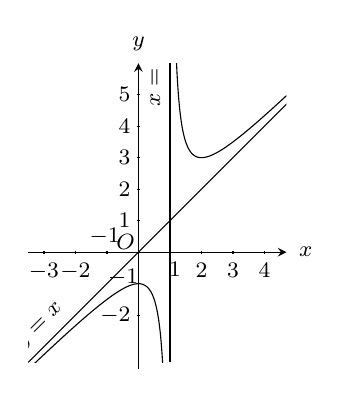
\begin{tikzpicture}[line cap=butt,line join=miter,>=stealth,scale=0.4,font=\footnotesize]
			\tikzset{declare function={xmin=-3.5;xmax=4.7;ymin=-3.5;ymax=6;},
				smooth,samples=450}
			\draw[->] (xmin,0)--(xmax,0) node[shift={(0:7pt)}]{$ x $};
			\draw[->] (0,ymin-.2)--(0,ymax) node[shift={(90:7pt)}]{$ y $};
			\fill (0,0) node[shift={(140:6pt)}]{$ O $};
			\clip (xmin,ymin) rectangle (xmax,ymax);
			\foreach \i in {-3,-2,2,3,4}{
				\draw(\i,1.5pt)--(\i,-1.5pt)node[below]{$\i$};}	
			\foreach \j in {-2,1,2,3,4,5}{
				\draw(-1.5pt,\j)--(1.5pt,\j) node[left]{$\j$};}
			\draw(-1.5pt,-1)--(1.5pt,-1)node[shift={(160:6.5pt)}]{$-1$};
			\draw(1,-1.5pt)--(1,1.5pt)node[shift={(-75:7pt)}]{$1$};
			\draw(-1,-1.5pt)--(-1,1.5pt)node[shift={(100:5pt)}]{$-1$};
			\def\f(#1){((#1)^2-(#1)+1)/((#1)-1)}
			\def\a{-1}
			\def\b{0}
			\def\c{0.5}
			\def\d{1.5}	
			\def\e{2}
			\def\g{3}	
			\pgfmathsetmacro\fa{\f(\a)}
			\pgfmathsetmacro\fb{\f(\b)}
			\pgfmathsetmacro\fc{\f(\c)}
			\pgfmathsetmacro\fd{\f(\d)}	
			\pgfmathsetmacro\fe{\f(\e)}
			\pgfmathsetmacro\fg{\f(\g)}	
			\draw[samples=100] plot[domain=-5.3:0.9] (\x,{\f(\x)});	
			\draw[samples=100] plot[domain=1.05:5.2] (\x,{\f(\x)});
			\draw[] (1,ymin)--(1,ymax) node [pos=0.95,sloped, above]{$x=1$};
			\draw[] (xmin,ymin)--(6,ymax) node [pos=0.08,sloped, above]{$y=x$};
	\end{tikzpicture}
	}
\loigiai{
}
\end{ex}

\begin{ex}
	\immini{Đồ thị hình bên là của một trong bốn hàm số sau. Hỏi đó là hàm số nào?
		\choice
		{$y=\dfrac{x^2-x}{x+1}$}
		{$y=\dfrac{x^2-3x}{x+1}$}
		{$y=\dfrac{x^2+1x+2}{x+1}$}
		{\True $y=\dfrac{-x^{2}}{x+1}$}}{
		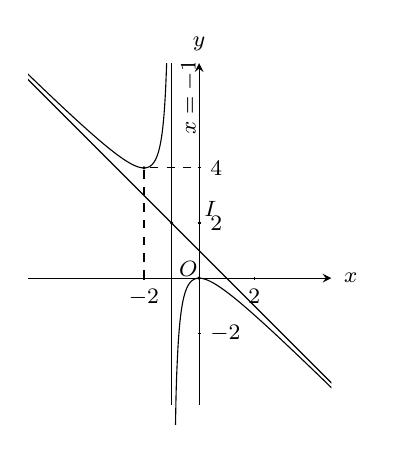
\begin{tikzpicture}[line cap=butt,line join=miter,>=stealth,scale=0.35,font=\footnotesize]
			\tikzset{declare function={xmin=-6.2;xmax=4.8;ymin=-4.6;ymax=7.8;},
				smooth,samples=450}
			\draw[->] (xmin,0)--(xmax,0) node[shift={(0:7pt)}]{$ x $};
			\draw[->] (0,ymin)--(0,ymax) node[shift={(90:7pt)}]{$ y $};
			\fill (0,0) node[shift={(140:5pt)}]{$ O $};
			\clip (xmin,ymin-.7) rectangle (xmax,ymax);
			\foreach \i in {-2,2}{
				\draw(\i,1.5pt)--(\i,-1.5pt)node[below]{$\i$};}
			\foreach \j in {-2,2,4}{
				\draw(-1.5pt,\j)--(1.5pt,\j) node[right]{$\j$};}	
			\def\f(#1){(-(#1)^2)/((#1)+1)} % Hàm số
			\def\q(#1){(-(#1)+1)} % Tiệm cận xiên
			\def\a{0}
			\def\b{-2}	
			\pgfmathsetmacro\fa{\f(\a)}
			\pgfmathsetmacro\fb{\f(\b)}	
			\draw[samples=250] plot[domain=-7.4:-1.1] (\x,{\f(\x)});	
			\draw[samples=250] plot[domain=-0.9:15] (\x,{\f(\x)});
			\draw[] plot [domain=-7.4:7] (\x,{\q(\x)}) ;
			\draw[] (-1,ymin)--(-1,ymax) node[sloped,pos=0.9,below] {$x=-1$};
			\foreach \x/\y in {\a/\fa,\b/\fb}{	
				\draw[dashed] (\x,0)|-(0,\y);}
			\foreach \x/\y in {\a/\fa,\b/\fb}{
				\fill[white,draw=black] (\x,\y) circle (1pt);}
			\fill[white,draw=black] (-1,2) circle (1pt) node[text=black,shift = {(14pt,5pt)}] {$I $};
		\end{tikzpicture}
	}
\loigiai{
}
\end{ex}

\begin{ex}
	\immini{Đồ thị hình bên là của một trong bốn hàm số sau. Hỏi đó là hàm số nào?
		\choice
		{$y=\dfrac{x^2-x+4}{x+1}$}
		{$y=\dfrac{x^2-2x+3}{x+1}$}
		{\True $y=\dfrac{-x^2-x+2}{x+1}$}
		{$y=\dfrac{x^2+x-1}{x+1}$}}{
		\begin{tikzpicture}[>=stealth, scale=0.35, font=\footnotesize]
			\draw[->] (-5,0)--(4.4,0) node[below] {$x$};
			\draw[->] (0,-5)--(0,6) node[left] {$y$};
			\draw[domain=-0.6:4, smooth] plot (\x, {-(\x)^2-(\x)+2)/(\x+1)});
			\draw[domain=-5:-1.35, smooth] plot (\x, {-(\x)^2-(\x)+2)/(\x+1)});
			\draw[domain=-5:4, smooth] plot (\x, {-\x});
			\draw (-1,-5)--(-1,6);
			\draw[fill=black] (0,0) node[below left=-0.1] {$O$} circle (1.2pt);
			\draw[fill=black] (1,0) node[below] {$1$} circle (1.2pt);
			\draw[fill=black] (-1,0) node[below left] {$-1$} circle (1.2pt);
			\draw[fill=black] (3,0) node[above] {$3$} circle (1.2pt);
			\draw[fill=black] (0,2) node[below left] {$2$} circle (1.2pt);
			\draw[fill=black] (0,-2.5) node[left] {$-\dfrac{5}{2}$} circle (1.2pt);
			\draw[dashed] (3,0)--(3,-2.5)--(0,-2.5) ;
			\end{tikzpicture}
	}
\loigiai{
}
\end{ex}

\begin{ex}
	\immini{Đồ thị hình bên là của một trong bốn hàm số sau. Hỏi đó là hàm số nào?
		\choice
		{$y=\dfrac{x^2+3}{x-1}$}
		{\True 	$y=\dfrac{x^{2}+x-3}{x-1}$}
		{$y=\dfrac{x^2-2x+3}{-x+1}$}
		{$y=\dfrac{x^2+3}{-x+1}$}}{
		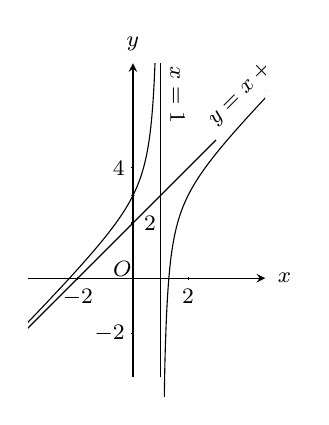
\begin{tikzpicture}[line cap=butt,line join=miter,>=stealth,scale=0.35,font=\footnotesize]
			\tikzset{declare function={xmin=-3.8;xmax=4.8;ymin=-3.6;ymax=7.8;},
				smooth,samples=450}
			\draw[->] (xmin,0)--(xmax,0) node[shift={(0:7pt)}]{$ x $};
			\draw[->] (0,ymin)--(0,ymax) node[shift={(90:7pt)}]{$ y $};
			\fill (0,0) node[shift={(140:5pt)}]{$ O $};
			\clip (xmin,ymin-.7) rectangle (xmax,ymax);
			\foreach \i in {-2,2}{
				\draw(\i,1.5pt)--(\i,-1.5pt)node[below]{$\i$};}
			\foreach \j in {-2,4}{
				\draw(-1.5pt,\j)--(1.5pt,\j) node[left]{$\j$};}	
			\draw(-1.5pt,2)--(1.5pt,2) node[right]{$2$};
			\def\f(#1){((#1)^2+(#1)-3)/((#1)-1)} % Hàm số
			\def\q(#1){((#1)+2)} % Tiệm cận xiên
			\def\a{0}	
			\pgfmathsetmacro\fa{\f(\a)}	
			\draw[samples=250] plot[domain=-7.4:0.9] (\x,{\f(\x)});	
			\draw[samples=250] plot[domain=1.1:15] (\x,{\f(\x)});
			\draw[] plot [domain=-7.4:7] (\x,{\q(\x)});
			\draw[] (1,ymin)--(1,ymax) node[rotate=180 ,pos=0.9,sloped,above] {$x=1$};
			\foreach \x/\y in {\a/\fa}{	
				\draw[dashed] (\x,0)|-(0,\y);}
			\foreach \x/\y in {\a/\fa}{
				\fill[white,draw=black] (\x,\y) circle (1pt);}
			;
			\node at (2.6,5.4) [rotate=45,right,fill=white]{$y=x+2$};
		\end{tikzpicture}
	}
\loigiai{
}
\end{ex}

\Closesolutionfile{ans}

\ind{PHẦN II.} \inden{Câu trắc nghiệm đúng sai. Trong mỗi ý a), b), c), d) ở mỗi câu, học sinh chọn đúng hoặc sai.}\\
\Opensolutionfile{ans}[ans/2D1-B4-d3-2]
\begin{ex}
	\immini{Cho hàm số $y=\dfrac{ax^2+bx+c}{mx+n}$ có đồ thị như hình bên.
	\choiceTF
	{Tập xác định của hàm số là $\mathbb{R}\backslash\{1\}$}
	{\True Hàm số nghịch biến trên khoảng $(-\infty;2)$ và $(2;+\infty)$}
	{\True Điểm $I(2;1)$ là tâm đối xứng của đồ thị}
	{\True Hệ số $a$ và $m$ trái dấu}}{
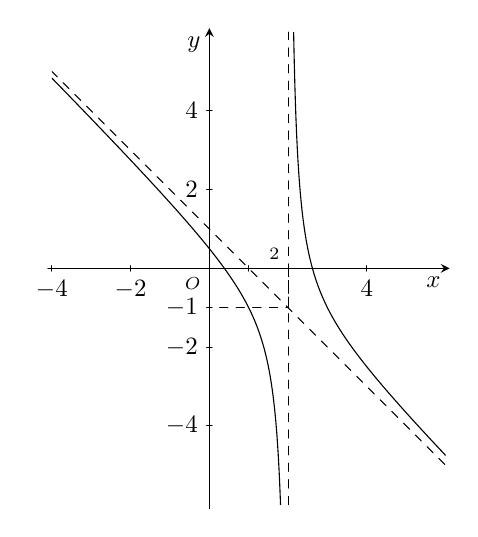
\begin{tikzpicture}[line join=round, line cap=round,>=stealth,x=0.5cm, y=0.5cm]
	\tikzset{every node/.style={scale=0.9}}
	\draw[->] (-4.1,0)--(6.1,0) node[below left] {$x$};
	\draw[->] (0,-6.1)--(0,6.1) node[below left] {$y$};
	\draw (0,0) node [below left] {\scriptsize$O$};
	\foreach \x/\nx in {-4/-4,-2/-2,1/ ,2/ ,4/4}
	\draw[thin] (\x,1pt)--(\x,-1pt) node [below] {$\nx$};
	\draw (2,0) node[above left]{\scriptsize$2$};
	\foreach \y/\ny in {-4/-4,-2/-2,-1/-1,2/2,4/4}
	\draw[thin] (1pt,\y)--(-1pt,\y) node [left] {$\ny$};
	\draw[dashed,thin](2,0)--(2,-1)--(0,-1);
	\draw[dashed,thin] (2,-6)--(2,6);
	\begin{scope}
		\clip (-4,-6) rectangle (6,6);
		\draw[samples=200,domain=-4:1.99,smooth,variable=\x] plot (\x,{(-1*((\x)^2)+3*(\x)+-1)/(1*(\x)+-2)});
		\draw[samples=200,domain=2.01:6,smooth,variable=\x] plot (\x,{(-1*((\x)^2)+3*(\x)+-1)/(1*(\x)+-2)});
		\draw[dashed,thin] (-6.1,7.1)--(6.1,-5.1);
	\end{scope}
\end{tikzpicture}}
\loigiai{
\begin{enumerate}[a)]
	\item 
	\item
	\item
	\item
\end{enumerate}}
\end{ex}

\begin{ex}
	\immini{Cho hàm số $y=\dfrac{ax^2+bx+c}{x+n}$ có đồ thị như hình bên.
		\choiceTF
		{\True Tập xác định của hàm số là $\mathbb{R}\backslash\{1\}$}
		{Điểm $I(1;2)$ là tâm đối xứng của đồ thị}
		{$a+2b=4$}
		{\True Đồ thị qua điểm $(2;10)$ khi $c=4$}}{
		\begin{tikzpicture}[line cap=round, line join=round,font=\footnotesize,>=stealth, scale=1,x=0.5cm, y=0.25cm]
			\tikzset{label style/.style={font=\footnotesize}}
			\draw[->] (-4,0)--(6,0) node[below] {$x$};
			\draw[->] (0,-8)--(0,15) node[left] {$y$};
			\draw[smooth, samples=100] plot[domain=-4:0.5] (\x, {  (2*(\x)^2-(\x)+4)/(\x-1) });
			\draw[smooth, samples=100] plot[domain=1.5:6] (\x, {  (2*(\x)^2-(\x)+4)/(\x-1) });
			\draw[dashed] (1,-8)node [right]{$x=1$}--(1,15) 
			plot[domain=-4:6](\x, {2*(\x)+1}) node[rotate=45,below]{$y=2x+1$};
	\end{tikzpicture}}
\loigiai{
	\begin{enumerate}[a)]
		\item
		\item
		\item
		\item
\end{enumerate}}
\end{ex}

\Closesolutionfile{ans}